
Mash-ups are applications generated by combining content, presentation or other applications functionalities from disparate sources. They aim to combine these sources to create useful new applications or services (the offer and consumption of data between two devices) to users. The LiveSync Tool combines videos from different sources with synchronization information from the Coupler Service to reproduce a synchronous presentation for these videos. The Mash-up Player is used to both presenting video synchronously and collecting the synchronization values. 

At the top of the interface all information necessary to the user as may be observed on Figure~\ref{menu_add_view}. Fallowing the orientations on the screen an user can select which videos want to watch, add a new videos, as well start the synchronization process for videos that he believes are not synchronized. 

\begin{figure}[h]
	\centerline{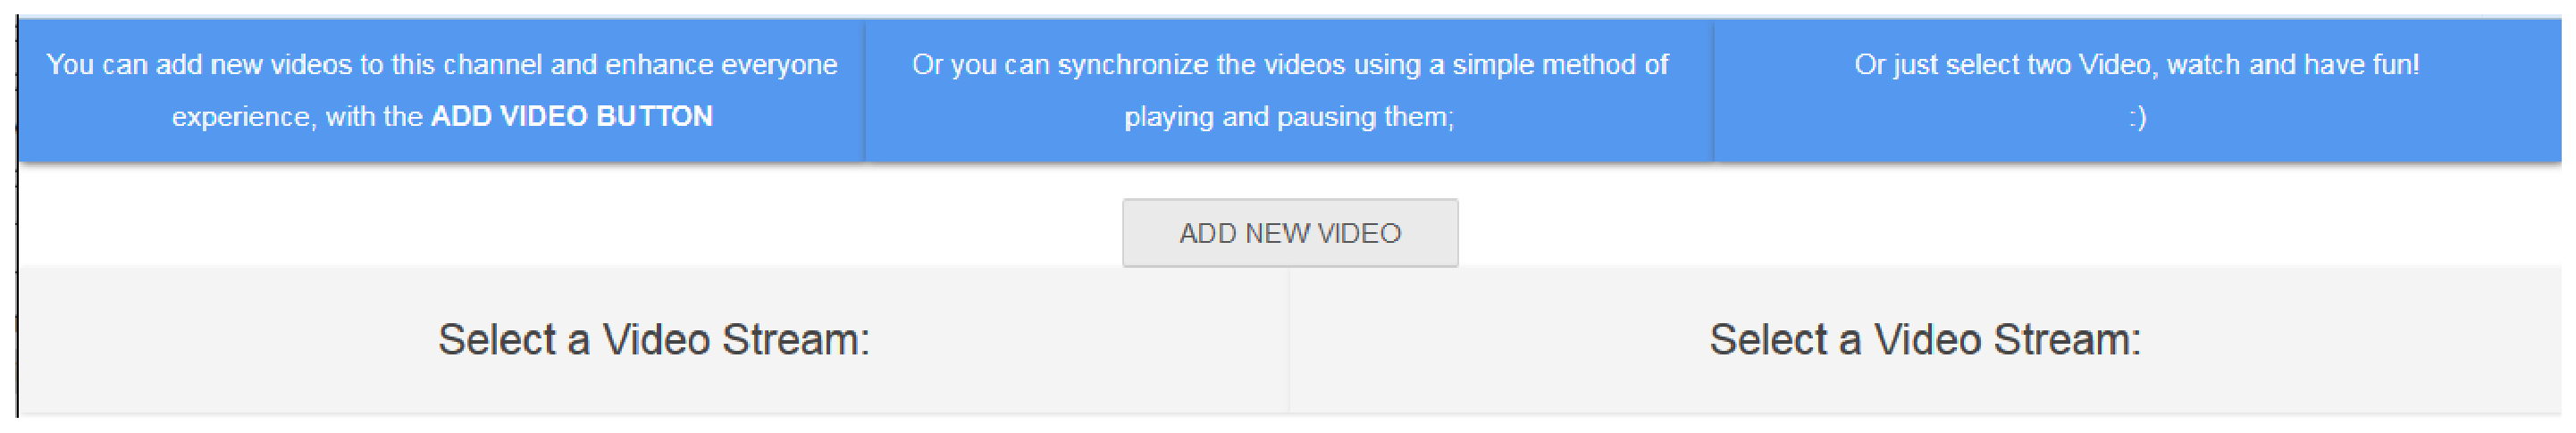
\includegraphics[scale=0.3] {figures/menu_add_view}}
	\caption{Action menu at the top of interface}
	\label{menu_add_view}
\end{figure}

When an user adds a video, an input text is shown to him, so he can add the video URI (WebSocket) or video ID YouTube). The page reloads and the new video is listed in the video list for everyone that connects to the application. Also, when the video is added by the user, an message is sent to the Coupler Service, containing the action to add a new video to the DAL, and the specification of it, such as label and URI.

When just playing two selected videos from the videos list, each for video player is created an instance that is compatible with that source (YouTube or WebSocket). Moreover, it is invisible to users where the video is coming from.

The last functionality of the mash-up is to synchronize the videos. When an user chooses to synchronizing a pair of videos, the mash-up display is reconfigured and the application enter in synchronization mode. LiveSync Tool uses a Play ’n Pause approach to synchronize the videos. Figure~\ref{live_tvs} represents the interface of the mash-up during a test: two cameras live streaming (content providers) a simulated television event to our mash-up application. Once the user decided the videos are synchronized he clicks on the done button, so his contribution committed to the Coupler Service that stores it into the DAL for further processing of the relation.

\begin{figure}[h!]
	\centerline{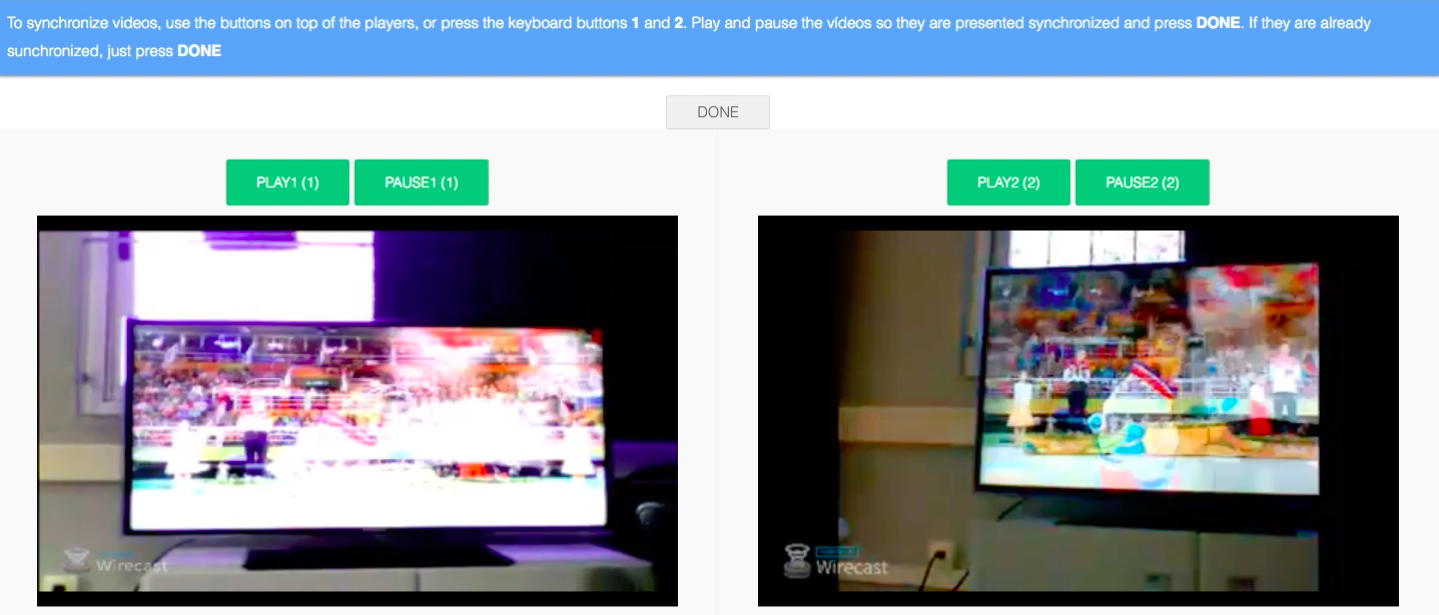
\includegraphics[scale=0.3] {figures/screen}}
	\caption{Live Streams from Olympic Games Synchronized through two different cameras}
	\label{live_tvs}
\end{figure}


